\subsection{Esercizio 7}
Le nuove funzioni utilizzate in  questo esercizio sono:
\begin{itemize}
    \item Metodo di Newton modificato
    \lstinputlisting[language=Matlab]{capitolo2/newtonmod.m}
    \item Metodo delle accelerazioni di Aitken
    \lstinputlisting[language=Matlab]{capitolo2/aitken.m}
\end{itemize}
La radice nulla della funzione $f(x)=x^2tan(x)$ ha molteplicità m = 3, in quanto $0$ annulla due volte il termine
$x^2$ e una volta il termine $tan(x)$. 

RISULTATI(raccolti in \nameref{cod:7}):

\begin{table}[h]
    \begin{tabular}{|l l l l l|}
            \hline
            Metodo & tolleranza$=10^{-3}$  & tolleranza$=10^{-6}$ & tolleranza$=10^{-9}$ & tolleranza$=10^{-12}$ \\
            \hline
            newton & 1.99400296195610$\cdot10^{-3}$ &  1.34922220938115$\cdot10^{-6}$  & 1.36940553054800$\cdot10^{-9}$ &  1.38989077859525$\cdot12$\\
            newton modificato  &  1.32348898008484$\cdot10^{-23}$ &   1.32348898008484$\cdot10^{-23}$  &  0  &  0\\
            aitken    &    3.72603946110722$\cdot10^{-24}$  &  3.72603946110722$\cdot24$  &  2.93579661656743$\cdot10^{-39}$ &   2.93579661656743$\cdot10{-39}$ \\
           \hline
    \end{tabular}
    \caption{valori approssimati da newton, newton modificato e aitken}
    \label{tab::2}     
    \end{table}
\newpage    
\begin{figure}[h]
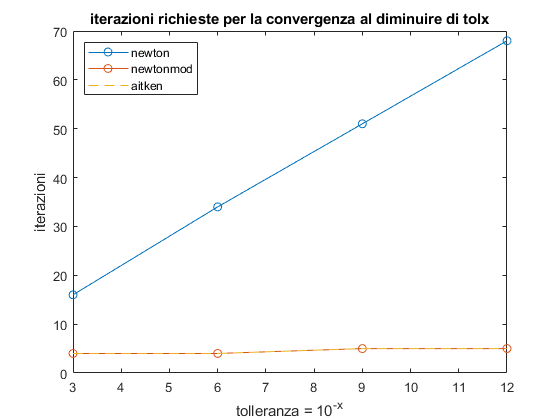
\includegraphics[scale=0.65]{capitolo2/iter2.png}
\caption{iterazioni richieste}
\label{fig::es6}
\end{figure}
Il metodo di newton classico perde la convergenza quadratica, essendo la radice cercata di molteplicità multipla. Il metodo di newton modificato e il metodo di aitken convergono
molto più rapidamente e newton modificato riesce anche a trovare la radice esatta.